\documentclass[__main__.tex]{subfiles}

\begin{document}

\qtitle{35}
Локальные В-сплайны второй степени, задача аппроксимации гладкой на отрезке функции с помощью таких сплайнов.\\

\begin{wrapfigure}{l!}{0.5\linewidth}
	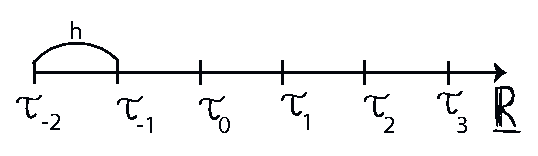
\includegraphics{35.eps}
	\label{35}
	\caption{ }
\end{wrapfigure}
Рассмотрим на прямой $\underline{\mathbb{R}}$ сетку\\ $B = \{\tau_m = hm + a\}, m \in \mathbb{Z}$(см. рис.\ref{35})\\
Для $i \in \mathbb{Z}_+$ определим функцию $S_i$:
$$
S_i(\tau) = x^2, \; x = \tau_i - \tau_{i-2}
$$
$B = \langle\tau_i = a + ih: i \in \mathbb{Z}\rangle$ - сетка на  $\mathbb{R}$\\
Для $i \in \mathbb{R}$ $B$ - сплайны 2-ой степени $S$ имеют вид (см.\ref{35})
\begin{gather*}
	S_i(\tau) = 
	\begin{cases}
		x^2, \;\; x = \frac{\tau - \tau_{i-2}}{\tau_{i-1} - \tau_{i-2}}, \;\; \tau \in [\tau_{i-2}; \tau_{i-1}]\\\\
		1 + 2x - x^2, \;\; x = \frac{\tau - \tau_{i-1}}{\tau_i - \tau_{i-1}}, \;\; \tau \in [\tau_{i-1}, \tau_i]\\\\
		2 - x^2, \;\; x = \frac{\tau - \tau_{i}}{\tau_{i+1} - \tau_{i}}, \;\; \tau \in [\tau_{i}, \tau_{i+1}]\\\\
		(1 - x)^2, \;\; x = \frac{\tau - \tau_{i+1}}{\tau_{i+2} - \tau_{i+1}}, \;\; \tau \in [\tau_{i+1}, \tau_{i+2}]\\\\
		0, \;\; \tau \notin [\tau_{i-2}, \tau_{i+2}]
	\end{cases}
\end{gather*}
\begin{center}
	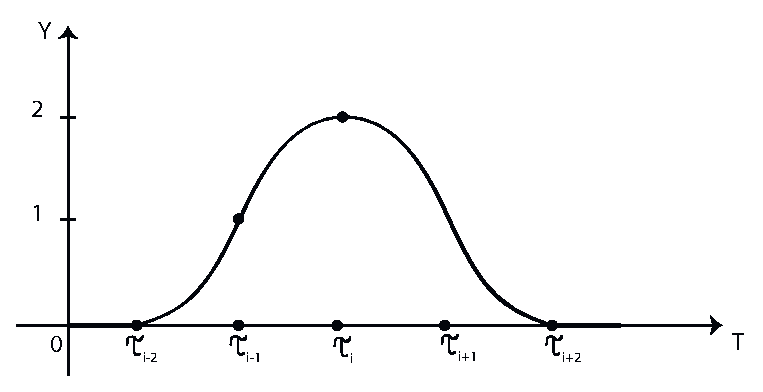
\includegraphics{35-par.eps}
	\label{35-par}
\end{center}
Для сетки $A = \langle a = \tau_0, \tau_1, .., \tau_k = b\rangle$ на $[a, b]$ для локальных $B$-сплайнов 2-ой степени $S_2(A)$ индуцируемых сеткой $A$ получаем базис $H = \langle h_0, h_1, ..., h_k \rangle$, где $h_i = S_i|_{[a, b]}$ для $i = \overline{0, k}$(см. рис) $S_2(A) = [H]$
\newpage
\begin{wrapfigure}[13]{l!}{0.45\linewidth}
	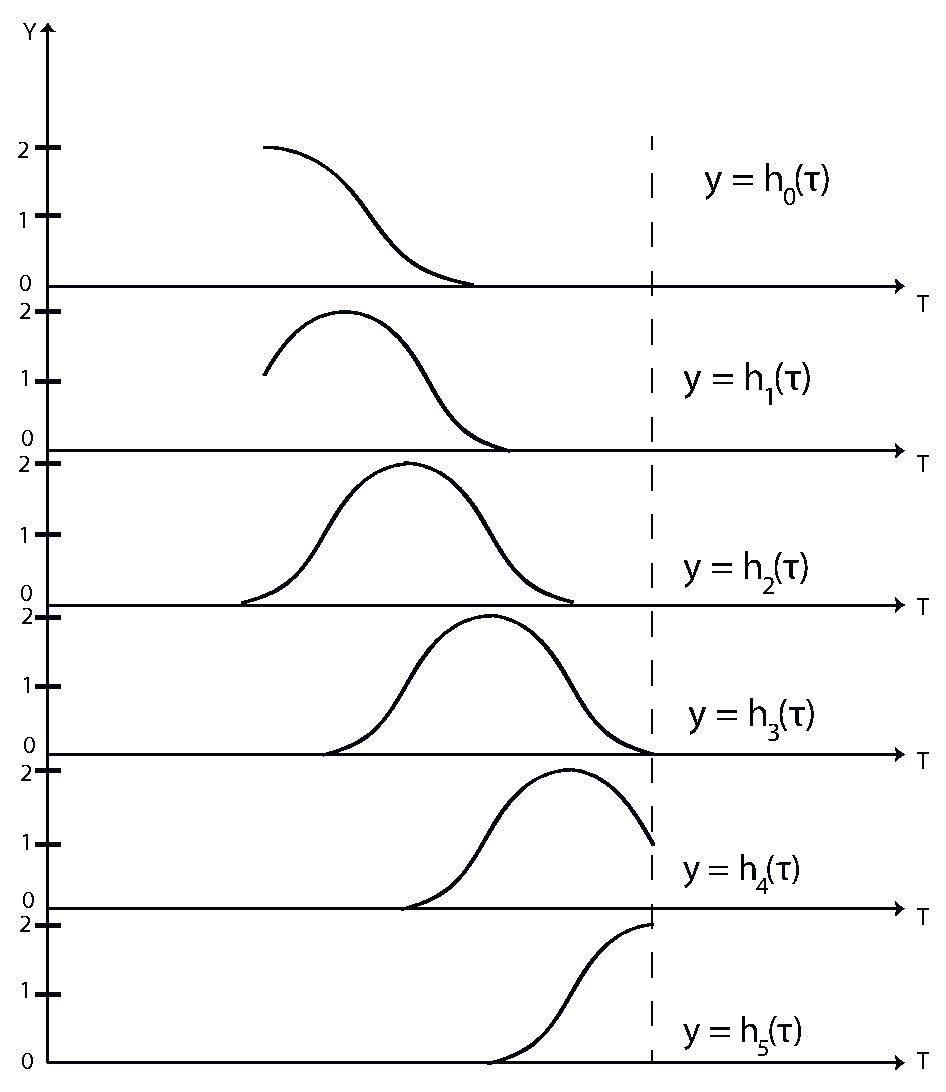
\includegraphics[scale=0.5]{35-multipar.eps}
	\label{35-multipar}
\end{wrapfigure}
Если на сетке задана $Α$-сеточная функция $^>y = [y_0, y_1, y_k\rangle \in\; ^> \mathbb{R}^{|A|}(A)$, то локальный $B$-сплайн 2-ой степени $S(A, \;^>y) \in S_2(A)$ представляется в виде:
\begin{gather}
\varphi = S_2(A, \;^>y) = \sum_{i=0}^{k}{z_iS_2(A, \;^>e_{i+1})},
\label{35-phi}
\end{gather}
где $(^>e_1, \;^>e_2, ..., \;^>e_{|A|})$ - стандартный базис $^>\mathbb{R}^{|A|}$ и $S_2(A, \;^>e_{i+1}) = h_i, i=\overline{0, k}$\\
Неизвестный вектор $^>z = [z_0, z_1, ..., z_k \rangle \in \;^>\mathbb{R}^{|A|}$  - коэффициенты в сплайне $\varphi = S_2(A, \;^>y)$ определяются из СЛАУ:
\begin{gather*}
	\begin{cases}
		z_0h_0(\tau_0) + z_1h_1(\tau_0) = y_0\\
		z_0h_0(\tau_1) + z_1h_1(\tau) + z_2h_2(\tau) = y_1\\
		...\\
		z_{k-2}h_{k-2}(\tau_{k-1}) + z_{k-1}h_{k-1}(\tau_{k-1}) + z_kh_h(\tau_{k-1}) = y_{k-1}\\
		z_{k-1}h_{k-1}(\tau_k) + z_kh_k(\tau_k) = y_k\\
	\end{cases}
\end{gather*}
\begin{gather*}
C = 
\begin{pmatrix}
	2 & 1 & 0 & ... & ... & 0\\
	1 & 2 & 1 & 0 & ...  & 0\\
	0 & ... & ... & ... & ... & ...\\
	... & ... & ... & ... & ... & ...\\
	0 & ... & ... & ... & ... & 0\\
	0 & ... & 0 & 1 & 2 & 1\\
	0 & ... & 0 & 0 & 1 & 2
\end{pmatrix}
\begin{pmatrix}
	z_0\\
	z_1\\
	.\\
	.\\
	.\\
	z_{k-1}\\
	z_{k}
\end{pmatrix}
=
\begin{pmatrix}
	y_0\\
	y_1\\
	.\\
	.\\
	.\\
	y_{k-1}\\
	y_{k}
\end{pmatrix}
\end{gather*}
\begin{gather}
C\;^>z = \;^>y,
\label{35-C}
\end{gather}
где $det(C) = k + 1 \ne 0$. Из \ref{35-C} определяется $^>z$. Следовательно, сплайны $S_2(A,\;^>y)$ из \ref{35-phi}\\

\end{document}